% Created: Enze Chen, May 2017
% Last edited: Enze Chen, December 2017
%
% Appendix B of the MSE 142 coursereader. This chapter reviews the math and physics a student ought to know when starting this course.
% Math: Differentiation, integration, and differential equations. 
% Physics: Forces, potential, simple harmonic motion.

% Uncomment the following three lines and last line to individually compile this chapter
%\documentclass[12pt, english]{book}
%\usepackage{142crstyle}
%\begin{document}

\chapter{Prerequisites} \label{ch:prereq}
%{ \doublespacing
Ideally, you should find most of the material in this section to be review. More advanced concepts will be developed as we go along, but just to make sure we are all starting on the same page, I have listed the major concepts that I expect my students to be familiar with coming into this course. It would be wise to skim this section and take some more time with concepts you might not be as familiar with---nailing those will allow you to get a lot more out of this course! If any of the following topics are confusing, please stop by office hours and I'd be happy to go over it. \par 

%%%%%%%%%%%%%%%%%%%%%%%%%%%%%%%%%%%%%%%%%%%%%%%%%%%%%%%%%%%%%%%%%%%%%%%%%%%%%%%%

\section{Math review} \label{sec:math}
\subsection{Complex numbers}
Quantum mechanics lives in complex space, and you will find yourself manipulating complex numbers quite frequently. A complex number is a number that can be expressed in the form 
\begin{tcolorbox}[title=Complex numbers]
$a + bi$, where $i = \sqrt{-1}$ and $a,b \in \mathbb{R}$
\end{tcolorbox}

We begin by looking at some powers of $i$. Namely,
\begin{align*}
i^1 &= \sqrt{-1} = i \\
i^2 &= i \cdot i = -1 \\
i^3 &= (i^2)i = -i \\
i^4 &= (i^3)i =  1 \\
i^5 &= (i^4)i = i \tag{same as $i^1$}\\
&\vdots 
\end{align*}
and so on, where we begin to see it repeating in the exponent modulo 4. When we look at negative exponents, the same pattern holds.
\begin{align*}
i^1 &= \sqrt{-1} = i \\
i^0 &= 1 \\
i^{-1} &= \dfrac{1}{i} = \dfrac{i}{i\cdot i} = -i \tag{same as $i^{3}$} \\
i^{-2} &= \dfrac{i^{-1}}{i} = \dfrac{-i}{i} = -1 \tag{same as $i^2$} \\
&\vdots 
\end{align*}

Whenever we want to eliminate complex numbers and work with real numbers instead, we multiply the complex number $a+bi$ by its \textbf{complex conjugate} $a-bi$, which has the opposite imaginary part. When we do so, we obtain 
\begin{equation*} 
(a+bi)(a-bi) = a(a) + a(-bi) + bi(a) + bi(-bi) = a^2 - \cancel{abi} + \cancel{abi} + b^2(-i^2) = a^2+b^2
\end{equation*}

Notation wise, if we have a complex number $\zeta = a + bi$, we denote its complex conjugate using an asterisk, such that $\zeta^* = a - bi$. \par

One of the most amazing results in complex analysis is \textbf{Euler's formula},~\footnote{See \href{https://en.wikipedia.org/wiki/Euler\%27s\_formula}{Wikipedia} for details and a proof.} which states that 
\begin{tcolorbox}[title=Euler's formula]
	$e^{ix} = \cos(x) + i\sin(x), \quad \forall x \in \mathbb{R}$
\end{tcolorbox}

When this formula is evaluated at $x=\pi$, we arrive at the identity $e^{i\pi} = \cos(\pi) + i\sin(\pi) = -1$. Euler's formula will be extremely useful in our analysis of waves, because the sinusoidal behavior of cosine and sine are all encompassed neatly in the complex exponential term. I'll give two final comments about Euler's formula here:
\begin{enumerate}[1.]
	\item Though it's written in a slightly different form, $e^{ix}$ is still a complex number, with $a = \cos(x)$ and $b = \sin(x)$. Therefore, it has a complex conjugate equal to $e^{-ix}=\cos(x) -i\sin(x)$. Let's apply what we did above and multiply $e^{ix}$ and $e^{-ix}$.
	\begin{align*}
	e^{ix} \cdot e^{-ix} &= (\cos(x) + i\sin(x))(\cos(x)-i\sin(x)) \\
	e^{ix} \cdot e^{-ix} &= \cos^2(x) -i\cos(x)\sin(x) + i\sin(x)\cos(x) -i^2\sin^2(x) \\
	e^{ix} \cdot e^{-ix} &= \cos^2(x) + \sin^2(x) \\
	\Aboxed{e^{ix} \cdot e^{-ix} &= 1} 
	\end{align*}
	
	We could have also arrived at this result by using the identity $e^a \cdot e^b = e^{a+b}$. Proceeding, $e^{ix} \cdot e^{-ix} = e^{ix - ix} = e^0 = 1$.
	
	\item With the complex conjugate on hand, we can now easily extract the individual cosine and sine terms. Notice what happens if we add $e^{ix}$ to $e^{-ix}$:
	\begin{align*}
	e^{ix} + e^{-ix} &= (\cos(x) + \cancel{i\sin(x)}) + (\cos(x) - \cancel{i\sin(x)}) \\
	e^{ix} + e^{-ix} &= 2\cos(x) \\
	\Aboxed{ \dfrac{e^{ix} + e^{-ix}}{2}&= \cos(x) }
	\end{align*}
	
	In a similar vein, we can show that $\boxed{\dfrac{e^{ix} - e^{-ix}}{2i} = \sin(x)}$ (note the $i$ in the denominator).
	
\end{enumerate}

%%%%%%%%%%%%%%%%%%%%%%%%%%%%%%%%%%%%%%%%%%%%%%%%%%%%%%%%%%%%%%%%%%%%%%%%%%%%%%%%

\subsection{Differentiation} \label{sec:diff}
No matter which form it takes, the \Sch\ equation is inherently a differential equation, so we should be prepared to work with derivatives in this course. Before jumping into the math, it's important to understand at a high level what a derivative represents. \par 
\begin{enumerate}[1.]
	\item Namely, the \textbf{first derivative} represents the slope of a tangent line to the function, or the instantaneous rate of change.
	\item The \textbf{second derivative} tells us the concavity of the function, where a positive value symbolizes concave up and a negative value for concave down.
\end{enumerate} 

\textbf{Note}: I will be using both $\dv{x} f$ and $f'$ notation for derivatives, so I kindly ask for your patience and flexibility. This might also be the first time you see the notation $\pdv{x} f$, which represents a \emph{partial} derivative of $f$ with respect to the variable $x$. We won't be working with them too much, but know that it behaves exactly the same way as a normal derivative would. It's written this way to clarify that the function $f$ depends on more variables than just $x$, and we would only like to know how it changes with respect to changes in $x$. \par 

The three main types of functions you will need to differentiate are:
\begin{enumerate}[1.]
	\item Polynomial: We apply the power rule, $\dv{x} x^n = nx^{n-1}$.
	\item Exponential: The derivative $ \dv{x} e^{f(x)} = f'(x)e^{f(x)}$.
	\item Trigonometric: $\dv{x} \cos(x) = -\sin(x)$. $\dv{x} \sin(x) = \cos(x)$. 
\end{enumerate}

In every case, watch out for 
\begin{itemize}
	\item Product rule: $\dv{x} [f(x)\cdot g(x)] = f(x)\cdot g'(x) + f'(x)\cdot g(x)$.
	\item Chain rule: $\dv{x} [f(g(x))] = f'(g(x)) \cdot g'(x)$.
\end{itemize}

%%%%%%%%%%%%%%%%%%%%%%%%%%%%%%%%%%%%%%%%%%%%%%%%%%%%%%%%%%%%%%%%%%%%%%%%%%%%%%%%

\subsection{Taylor series}

Derivatives involve infinitesimals, and one technique that we will apply (and you will master!) is taking \textbf{Taylor series}~\footnote{See \href{http://tutorial.math.lamar.edu/Classes/CalcII/TaylorSeries.aspx}{Paul Dawkins' page} for more information.} expansions of functions. We will rely on Taylor series heavily to make approximations of functions whenever the result approaches 0. The Taylor series of a function $f(x)$ at a point $x=a$ is given by the infinite power series:
\begin{tcolorbox}[title=Taylor series formula]
$f(x)|_{x=a} = f(a) + f'(a)(x-a) + \dfrac{f''(a)}{2!}(x-a)^2 + \dots = \displaystyle\sum_{n=0}^{\infty} \dfrac{f^{(n)}(a)}{n!}(x-a)^n$
\end{tcolorbox}

The \emph{order} of a Taylor series is the largest degree polynomial in the series expansion that we write out explicitly. Everything above the highest-order term is typically discarded or abbreviated using $\text{big O}$ notation. As an example, the Taylor series for cosine about $x=0$ can be expressed as \[ \cos(x)|_{x=0} = 1 - \dfrac{x^2}{2!} + \order{x^4} \] where we lumped together everything after the second order term because those values are small enough that they won't affect the final answer and can be safely discarded. There's no requirement to memorize any specific Taylor series expansions for this class; you should just look them up in a table or derive the first few terms (we generally don't go beyond second order terms).

%%%%%%%%%%%%%%%%%%%%%%%%%%%%%%%%%%%%%%%%%%%%%%%%%%%%%%%%%%%%%%%%%%%%%%%%%%%%%%%%

\subsection{Integration}
This course will feature plenty of integrals, not all of which are intuitive, but we will walk through all of them in lecture. As long as you have solid fundamentals, and are able to keep track of signs, integration limits, etc., then they shouldn't present a problem. \par 

One thing to keep in mind for integration, differentiation, and this course in general is the idea of \emph{linear} operations/operators. What this essentially means is that we can distribute the operation across a sum, with integration being an example:
\begin{tcolorbox}[title=Linear operations---integration example]
	$\displaystyle\int \left[ f(x) + g(x) + h(x) \right]\dd{x} = \displaystyle\int f(x)\dd{x} + \displaystyle\int g(x)\dd{x} + \displaystyle\int h(x)\dd{x}$
\end{tcolorbox}

%%%%%%%%%%%%%%%%%%%%%%%%%%%%%%%%%%%%%%%%%%%%%%%%%%%%%%%%%%%%%%%%%%%%%%%%%%%%%%%%

\subsection{Differential equations}
Knowledge of basic differential equations can be helpful for this course, but we will be sure to cover all the bases. Just know that a differential equation such as the \Sch\ equation combines all the fun of differentiation with the fun of integration! A differential equation always features some combination of derivatives, variables, and constants, an example of which is given by \[ \dv{y}{x} + f(x)y = 0 \] 
where $f(x)$ is some arbitrary function that only depends on $x$. To cover some basic terminology, the above equation is a \textbf{linear}, \textbf{first-order} differential equation because the derivatives of $y$ (our dependent variable) are not multiplied together (only added) and the highest-order derivative of $y$ is the first derivative. This equation is also \textbf{separable} because we are able to rearrange the equation to have all variables of the same type on each side of the equation.
\begin{align*}
\dv{y}{x} + f(x)y &= 0 \\
\dv{y}{x} &= -f(x)y \\
\frac{1}{y}\dd{y} &= -f(x)\dd{x}
\end{align*}

Separable differential equations are nice for many reasons, one of which is that they can be solved by straightforward integration. We proceed to get
\begin{align*}
\int\frac{1}{y}\dd{y} &= \int-f(x)\dd{x} \\
\ln y &= -\int f(x)\dd{x} + C \\
y &= y_0\exp\left(-\int f(x)\dd{x}\right)
\end{align*}

where $y_0$ appears as the integration constant depending on initial conditions. We won't be focusing too much on solving differential equations in this class, at least not in this way, and this example was just meant to give you a general idea for the procedure.

%%%%%%%%%%%%%%%%%%%%%%%%%%%%%%%%%%%%%%%%%%%%%%%%%%%%%%%%%%%%%%%%%%%%%%%%%%%%%%%%

\section{Physics review}
Often times, it helps to reframe the abstract nature of quantum mechanics in a classical mechanics context, so this section will highlight some key points in classical mechanics and electromagnetism. \par 

\subsection{Forces and potentials}

Newton's laws of motion are fundamentally important, and you should be familiar in particular with the Second law, which says that force equals mass times acceleration.
\begin{tcolorbox}[title=Newton's Second law] \vspace{-2ex}
\[ F = ma = m \dv{v}{t} = m\dv[2]{x}{t} \]
\end{tcolorbox} 

This expression can be rearranged to obtain 
\begin{equation*}
	F = m\dv{v}{t} \implies \int F\dd{t} = \int m\dd{v} \implies \boxed{p = mv}
\end{equation*}
where $p$ is the symbol for \textbf{momentum}. \par 

We can also find the energy/work done by multiplying together force and distance, such that $\Delta U = -W = -F \Delta x$. In differential terms, this is commonly expressed as 
\begin{equation}
\boxed{F = -\dv{U}{x}} \label{eq:FdU}
\end{equation}
where the direction of the force is opposite the energy gradient (e.g. a hill slopes upwards, but pushes a ball downwards). \par 

You should already know the expressions for the different forms of energy, shown in the table below. \par 
\begin{table}[!h]
	\centering 
	\begin{tabular}{ll}
		\textbf{Form} & \textbf{Expression} \\ \toprule 
		Gravitational potential energy & $U_g = mgh$ \\ \rule{0ex}{3ex}
		Elastic potential energy & $U_e = \frac{1}{2}kx^2$ \\ \rule{0ex}{3ex}
		Kinetic energy & $K = \frac{1}{2}mv^2$
	\end{tabular}
\end{table} 

%%%%%%%%%%%%%%%%%%%%%%%%%%%%%%%%%%%%%%%%%%%%%%%%%%%%%%%%%%%%%%%%%%%%%%%%%%%%%%%%

\subsection{Simple harmonic motion} \label{sec:shm}
The behavior of atoms and subatomic particles can often be modeled using harmonic oscillators, so it's important to start with a solid understanding of simple harmonic motion (SHM) and the simple harmonic oscillator (SHO). 

\begin{figure}[!h]
	\centering
	\begin{tikzpicture}
	\node[draw, rectangle, minimum size=8mm] (m) at (2.9,0) {$m$};
	\draw[decoration={aspect=0.45, segment length=3mm, amplitude=3mm,coil},decorate] (0,0)--(m); 
	\fill[pattern = north east lines] (0,-0.42) rectangle (-0.4,1);
	\draw[thick] (0,1)--(0,-0.42)--(3.5,-0.42);
	\end{tikzpicture}
	\caption{Model of a simple harmonic oscillator as a mass on a spring.}
	\label{fig:SHO-model}
\end{figure} 

We can think of a SHO as a mass on a spring (Figure~\ref{fig:SHO-model}). In equilibrium, everything is stationary; but when the mass is perturbed slightly, it feels a restoring force from the spring given by \textbf{Hooke's Law}: $F=-kx$, where $k$ is the spring constant and $x$ is the amount of displacement from equilibrium. The elastic potential energy stored in the spring is given by $U_e=\frac{1}{2}kx^2$, which can be derived by integrating Hooke's Law according to Equation~\ref{eq:FdU}. \par 

With SHM, we typically like to think of cycles in terms of angle traversed, which makes it easier to model using trigonometric functions. This leads to \textbf{angular frequency}, $\omega$, which has units of radians per second (rad/s). In terms of the cycle frequency $f$, we have $\omega = 2\pi f$. Since period is the inverse of frequency, this also leads to $\omega = \frac{2\pi}{T}$. Perhaps most importantly, we can relate the angular frequency to the spring constant and mass by 
\begin{tcolorbox}[title=Key Relationship] \vspace*{-2ex}
\begin{equation}
\omega=\sqrt{\frac{k}{m}} \label{eq:wkm}
\end{equation}
\end{tcolorbox}

We will not derive Equation~\ref{eq:wkm} here, but we will apply the result often when analyzing the quantum harmonic oscillator.

%%%%%%%%%%%%%%%%%%%%%%%%%%%%%%%%%%%%%%%%%%%%%%%%%%%%%%%%%%%%%%%%%%%%%%%%%%%%%%%%

\subsection{Electromagnetism}
Then we have the electromagnetic analog to mechanics. As we analyze the behavior of electrons, we will treat them as point charges $q$ that experience a force given by 
\begin{equation*}
	F = qE = -q\dv{V}{x}
\end{equation*}

where $E$ is the electric field and $V$ is the electric potential. Similar to the gravitational context, the force is related to the electric potential energy by $F = -\dv{U}{x}$, and an electron with mass $m_e$ experiences an acceleration according to Newton's Second law, $F = m_ea$. When dealing with two point charges, the force is also given by \textbf{Coulomb's law}, an inverse-square law which states that
\begin{equation*}
	F = \frac{1}{4\pi \varepsilon_0} \frac{q_1q_2}{r^2}
\end{equation*}

where $\varepsilon_0$ is the permittivity of free space, $q_1$ and $q_2$ are the charges of the particles, and $r$ is the distance between them. \par 

It may also be helpful to know that light is one form of electromagnetic radiation, and the force carrier for the electromagnetic force is called the \textbf{photon}. Traveling electromagnetic radiation has both an electric field and magnetic field that are orthogonal (perpendicular) to each other (Figure~\ref{fig:EB-field}). The \emph{frequency} of light is directly proportional to its energy and the range of frequencies of electromagnetic radiation make up the \textbf{electromagnetic spectrum} (Figure~\ref{fig:EM-spec}).

\begin{figure}[!h]
	\centering
	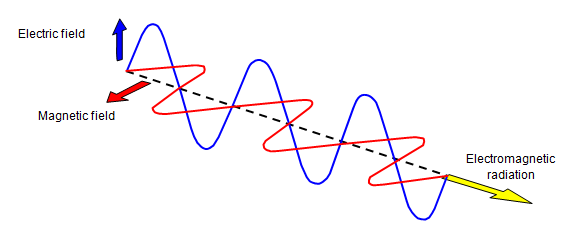
\includegraphics[width=0.7\linewidth]{EB-field}
	\caption{Electromagnetic radiation contains orthogonal electric and magnetic fields. Image courtesy of \href{http://www.schoolphysics.co.uk/age16-19/Wave\%20properties/Polarisation/text/Polarisation_/images/2.png}{schoolphysics}.}
	\label{fig:EB-field}
\end{figure}

\begin{figure}[!h]
	\centering
	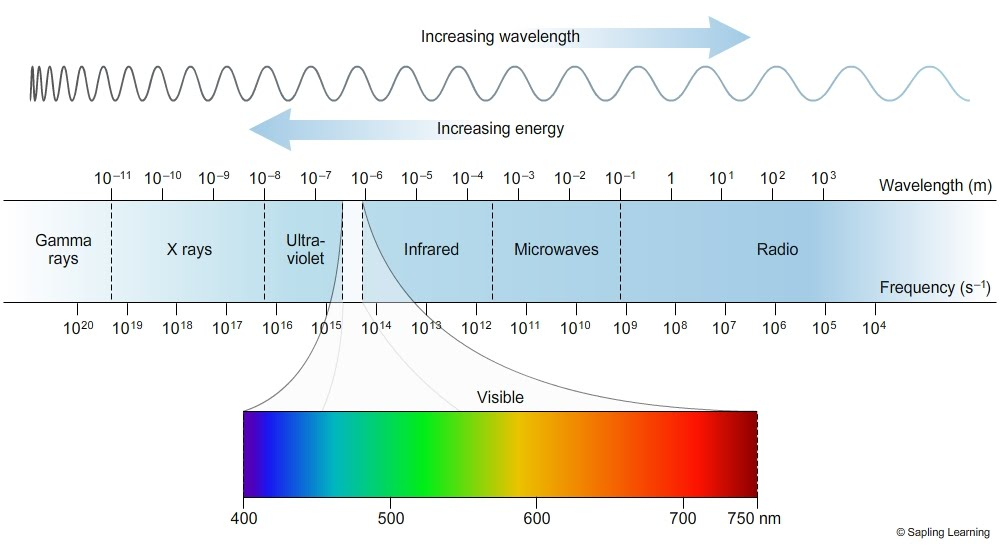
\includegraphics[width=0.9\linewidth]{EM-spectrum}
	\caption{The electromagnetic spectrum. Image courtesy of \href{https://sites.google.com/site/chempendix/em-spectrum}{Sapling Learning}.}
	\label{fig:EM-spec}
\end{figure}

%}
%\end{document}